\chapter{Portata delle interazioni}

Nel capitolo precedente, costruendo il modello a goccia, siamo partiti da un unico fatto sperimentale: l'energia di legame per nucleone è pressoché costante. Da lì abbiamo dedotto che la densità nucleare è la stessa per tutti i nuclei e che quindi l'interazione nucleare deve essere \emph{a corto raggio}, cioè che ciascun nucleone interagisce soltanto con i propri vicini. Questa proprietà è l'assunzione su cui poggia l'intera formula semiempirica.

Non ne abbiamo però mai spiegato l'origine. Abbiamo cioè stabilito che la forza nucleare si spegne a una certa distanza, ma non perché, né quanto valga quella distanza.\\

C'è poi una seconda questione, apparentemente slegata, rimasta altrettanto aperta. Nella formula semiempirica il termine coulombiano è l'unico a crescere come $Z^2$ anziché come $A$, e proprio per questo finisce per dominare nei nuclei pesanti, nonostante abbia il coefficiente più piccolo di tutti. Avevamo osservato il fatto senza giustificarlo: perché la repulsione elettrica, a differenza dell'attrazione nucleare, non satura?\\

Le due domande hanno la stessa risposta, e questo capitolo serve a ricavarla: \emph{La portata di una forza è fissata dalla massa della particella che la media}.

Un mediatore massivo produce una forza che si spegne esponenzialmente oltre una distanza $\lambda = \hbar/mc$; un mediatore privo di massa produce una forza di portata infinita. L'interazione nucleare è mediata dal pione, che ha massa, e la distanza che ne risulta è dell'ordine del fermi, cioè esattamente la scala $r_0$ usata nel modello a goccia. L'interazione elettromagnetica è mediata dal fotone, privo di massa, e per questo ogni protone del nucleo sente tutti gli altri e non solo i vicini: da qui il $Z^2$.\\

Il percorso sarà il seguente. Introdurremo anzitutto il potenziale di Yukawa, cioè la forma più semplice di potenziale dotato di una scala di lunghezza, assumendola per il momento come un'ipotesi. Studieremo poi la relazione di dispersione di una particella massiva, trovando che nel regime statico il numero d'onda diventa \emph{immaginario} e l'onda, invece di propagarsi, decade esponenzialmente nello spazio: è questa l'origine della scala di lunghezza. Modificheremo quindi le equazioni di Maxwell in modo che descrivano un ipotetico fotone dotato di massa, e risolvendole per una carica puntiforme ritroveremo il potenziale di Yukawa, questa volta non come ipotesi ma come conseguenza. Vedremo infine come questa ipotesi si possa mettere alla prova sperimentalmente, misurando con grande precisione il comportamento di una carica all'interno di un conduttore.

Si noti che nel seguito non stiamo descrivendo l'interazione nucleare con le equazioni di Maxwell. Il conto viene svolto nel caso elettromagnetico perché è l'unico campo di cui conosciamo già le equazioni, ma ciò che ricaveremo non dipende dalla natura del campo: discende unicamente dalla relazione di dispersione relativistica e vale per qualunque campo i cui quanti abbiano massa. Di questa sezione trasporteremo al caso nucleare soltanto il risultato strutturale, cioè il legame fra la massa del mediatore e la portata della forza.

Il risultato tornerà utile anche più avanti. Nel capitolo sul decadimento $\alpha$ la particella dovrà attraversare una barriera di potenziale fatta di due pezzi molto diversi fra loro: un'attrazione nucleare che si interrompe bruscamente al raggio di contatto e una repulsione coulombiana che si estende per decine di fermi. È la differente portata delle due interazioni a dare alla barriera quella forma, e senza di essa il decadimento $\alpha$ non esisterebbe come fenomeno osservabile.

\section{Potenziale di Yukawa}

Dato che l'interazione nucleare è a corto raggio, per quanto abbiamo dedotto costruendo il modello a goccia, deve esistere una distanza caratteristica oltre la quale questa interazione si spegne. Il modo più semplice per descrivere un potenziale dotato di una scala di lungezza $\lambda$ è il potenziale di Yukawa.\mkeyword{potenziale di Yukawa}
%
\begin{tcolorbox}[colback=yellow!10!white, colframe=orange!70!black, boxrule=0.8pt]
\begin{equation}
    V_Y(r) = g \cdot \frac{e^{-\mu r}}{r} = g \cdot \frac{e^{-r/\lambda}}{r} \qquad , \qquad \lambda = \frac{1}{\mu}
    \label{eq:yukawa}
\end{equation}
\end{tcolorbox}
che si comporta nei due regimi come
%
\begin{equation*}
    V_Y \simeq \frac{g}{r} \ \ \text{per} \ \ \frac{r}{\lambda} \ll 1 \qquad , \qquad V_Y \to 0 \ \ \text{per} \ \ \frac{r}{\lambda} \gg 1
\end{equation*}
A distanze molto minori della scala caratteristica l'esponenziale vale circa $1$ e si recupera il potenziale coulombiano; a distanze maggiori il potenziale viene tagliato via esponenzialmente.

\begin{figure}[htbp]
\centering
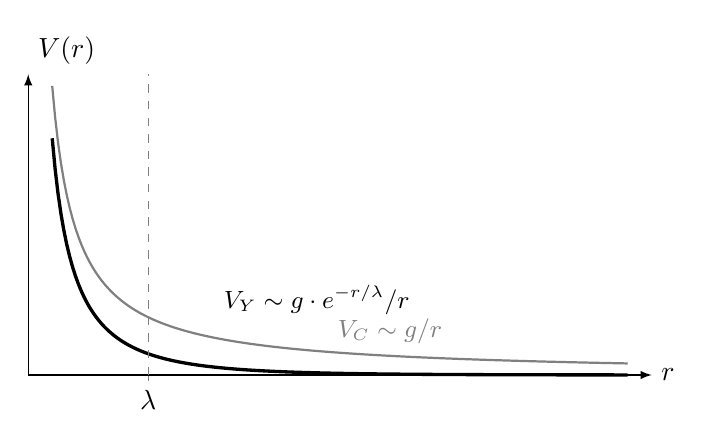
\begin{tikzpicture}
\begin{axis}[
    width=9.5cm, height=5.4cm,
    axis lines=left, axis line style={-latex},
    xlabel={$r$}, ylabel={$V(r)$},
    xlabel style={at={(ticklabel* cs:1)}, anchor=west},
    ylabel style={at={(ticklabel* cs:1)}, anchor=south west, rotate=-90},
    xmin=0, xmax=5.2, ymin=0, ymax=5.2,
    xtick={1}, xticklabels={$\lambda$}, ytick=\empty,
    clip=false,
]
\addplot[gray, thick, domain=0.2:5, samples=200] {1/x};
\node[anchor=west, font=\small, gray] at (axis cs:2.5,0.75) {$V_C \sim g/r$};
\addplot[black, very thick, domain=0.2:5, samples=200] {exp(-x)/x};
\node[anchor=west, font=\small] at (axis cs:1.55,1.3) {$V_Y \sim g \cdot e^{-r/\lambda}/r$};
\draw[dashed, gray] (axis cs:1,0) -- (axis cs:1,5.2);
\end{axis}
\end{tikzpicture}
\caption{Potenziale di Yukawa}
\label{fig:yukawa}
\end{figure}

La domanda naturale è da dove venga quell'esponenziale. Di seguito andremo a ricavare questa forma, la quale è generale e applicabile a più tipi di forze, dall'interazione Coulombiana, ipotizzando che essa sia mediata da una particella massiva\footnote{Sfrutteremo l'interazione coulombiana solo per un fatto di praticità, in quanto, grazie alle equazioni di Maxwell, sappiamo trattare perfettamente interazioni elettromagnetiche. Questo non vuol dire che l'interazione nucleare abbia natura elettromagnetica, vuol solo dire che il legame fra la massa del mediatore e la portata della forza è lo stesso in entrambi i casi.}.

\subsection{Mediatore massivo}

Per la particella libera vale la relazione relativistica 
%
\begin{equation*}
    E^2 = p^2 c^2 + m^2 c^4
\end{equation*}
e, dal punto di vista ondulatorio, $E = \hbar \omega$ e $\mathbf{p} = \hbar \mathbf{k}$. Sostituendo si ottiene la relazione di dispersione 
% 
\begin{equation}
    \omega^2 = c^2(k^2 + \mu^2) \quad , \quad \mu = \frac{mc}{\hbar}
\label{eq:particella_massiva}
\end{equation}
Per $m = 0$ si ritrova $\omega^2 = c^2 k^2$, cioè le onde elettromagnetiche che nel vuoto si propagano alla velocità della luce. 

Se invece la particella ha massa, la \eqref{eq:particella_massiva} ha due conseguenze. 

\textbf{Le velocità dipendono dalla frequenza.} La velocità di fase vale
%
\begin{equation}
    v_\varphi = \frac{\omega}{k} = \frac{c \, \omega}{\sqrt{\omega^2 - c^2\mu^2}} > c
\end{equation}
ma questo non costituisce un problema, perché la velocità di fase non trasporta informazione. Quella che conta è la velocità di gruppo
%
\begin{equation}
    v_g = \frac{\partial \omega}{\partial k} = \frac{c^2 k}{\omega} = c\sqrt{1 - \frac{c^2\mu^2}{\omega^2}} \simeq c\left(1 - \frac{c^2\mu^2}{2\omega^2}\right) < c
\end{equation}
che risulta correttamente minore di $c$. Si noti che $v_\varphi v_g = c^2$. La conseguenza osservabile è che fotoni di energia diversa viaggerebbero a velocità diverse: non si muoverebbero tutti a $c$, e un lampo di luce proveniente da una sorgente lontana arriverebbe disperso nel tempo a seconda del colore.\\

\textbf{Nel regime statico il numero d'onda diventa immaginario.} Ponendo $\omega = 0$ nella \eqref{eq:dispersione} si ottiene
%
\begin{equation*}
    k^2 + \mu^2 = 0 \qquad \Longrightarrow \qquad k^2 = -\mu^2 \qquad \Longrightarrow \qquad k = \pm i\mu
\end{equation*}
e l'onda piana diventa
%
\begin{equation}
    e^{-i\omega t} e^{ikz} \ \longrightarrow \ e^{-i\omega t} e^{i(i\mu)z} = e^{-i\omega t} e^{-\mu z}
\end{equation}
cioè un'onda che non oscilla nello spazio ma decade esponenzialmente, con portata $\lambda = 1/\mu$. È esattamente la scala del potenziale di Yukawa.\\

\subsection{Equazioni di Maxwell per fotone massivo}

Vediamo adesso come modificare le equazioni di Maxwell perché valga la \eqref{eq:particella_massiva}. 
%
\begin{equation*}
\begin{aligned}
    \text{i.} \ \ \mathbf{\nabla}\cdot\mathbf{E} &= 4\pi\rho  &\qquad \text{iii.} \ \ \mathbf{\nabla}\cdot\mathbf{B} &= 0 \\
    \text{ii.} \ \ \mathbf{\nabla}\times\mathbf{E} + \frac{1}{c}\frac{\partial \mathbf{B}}{\partial t} &= 0 &\qquad \text{iv.} \ \ \mathbf{\nabla}\times\mathbf{B} - \frac{1}{c}\frac{\partial \mathbf{E}}{\partial t} &= \frac{4\pi}{c}\mathbf{J}
\end{aligned}
\end{equation*}
cui si affiancano le definizioni dei potenziali
%
\begin{equation}
    \mathbf{E} = -\mathbf{\nabla}\varphi - \frac{1}{c}\frac{\partial \mathbf{A}}{\partial t} \qquad , \qquad \mathbf{B} = \mathbf{\nabla}\times\mathbf{A}
    \label{eq:potenziali}
\end{equation}

Inserendo la prima delle \eqref{eq:potenziali} nella i. e la seconda nella iv. si ottiene, nel vuoto,
%
\begin{equation*}
    \mathbf{\nabla}\cdot\left(-\mathbf{\nabla}\varphi - \frac{1}{c}\frac{\partial \mathbf{A}}{\partial t}\right) = 0 \qquad , \qquad \mathbf{\nabla}\left(\mathbf{\nabla}\cdot\mathbf{A}\right) - \nabla^2 \mathbf{A} + \frac{1}{c}\mathbf{\nabla}\frac{\partial \varphi}{\partial t} + \frac{1}{c^2}\frac{\partial^2 \mathbf{A}}{\partial t^2} = 0
\end{equation*}
e scegliendo la gauge di Lorenz\mkeyword{gauge di Lorenz}
%
\begin{equation*}
    \mathbf{\nabla}\cdot\mathbf{A} + \frac{1}{c}\frac{\partial \varphi}{\partial t} = 0
\end{equation*}
le due equazioni si disaccoppiano in
%
\begin{equation}
\begin{cases}
    -\nabla^2 \varphi + \dfrac{1}{c^2}\dfrac{\partial^2 \varphi}{\partial t^2} = 0 \\[8pt]
    -\nabla^2 \mathbf{A} + \dfrac{1}{c^2}\dfrac{\partial^2 \mathbf{A}}{\partial t^2} = 0
\end{cases}
\end{equation}
Dato che possiamo scrivere qualsiasi potenziale come sovrapposizione di onde piane, poniamo $\varphi = \varphi_0 e^{i(\mathbf{k}\cdot\mathbf{r} - \omega t)}$ e $\mathbf{A} = \mathbf{A}_0 e^{i(\mathbf{k}\cdot\mathbf{r}-\omega t)}$ e quindi si ottiene
%
\begin{equation*}
    -k^2 + \frac{\omega^2}{c^2} = 0
\end{equation*}
cioè la relazione di dispersione di una particella \emph{senza} massa.\\

Noi vogliamo invece $-k^2 + \omega^2/c^2 - \mu^2 = 0$. Questo significa che le equazioni d'onda devono diventare
%
\begin{equation}
\begin{cases}
    -\nabla^2 \varphi + \dfrac{1}{c^2}\dfrac{\partial^2 \varphi}{\partial t^2} = -\mu^2 \varphi \\[8pt]
    -\nabla^2 \mathbf{A} + \dfrac{1}{c^2}\dfrac{\partial^2 \mathbf{A}}{\partial t^2} = -\mu^2 \mathbf{A}
\end{cases}
\end{equation}
da cui si ricavano le equazioni di Maxwell per il fotone massivo

\begin{tcolorbox}[colback=yellow!10!white, colframe=orange!70!black, boxrule=0.8pt]
\begin{equation}
\begin{aligned}
    \text{i.} \ \ \mathbf{\nabla}\cdot\mathbf{E} &= 4\pi\rho - \mu^2 \varphi  &\qquad \text{iii.} \ \ \mathbf{\nabla}\cdot\mathbf{B} &= 0 \\
    \text{ii.} \ \ \mathbf{\nabla}\times\mathbf{E} + \frac{1}{c}\frac{\partial \mathbf{B}}{\partial t} &= 0 &\qquad \text{iv.} \ \ \mathbf{\nabla}\times\mathbf{B} - \frac{1}{c}\frac{\partial \mathbf{E}}{\partial t} &= \frac{4\pi}{c}\mathbf{J} - \mu^2 \mathbf{A}
\end{aligned}
\end{equation}
\end{tcolorbox}
Si noti che soltanto le due equazioni \emph{inomogenee} vengono modificate. Le altre due non possono cambiare, perché non sono leggi fisiche indipendenti ma identità matematiche che discendono dalle definizioni \eqref{eq:potenziali}: la divergenza di un rotore è nulla e il rotore di un gradiente è nullo. Si noti anche che il termine di massa coinvolge esplicitamente i potenziali, cosa che rompe l'invarianza di gauge.

\newpage

\subsection{Il potenziale di una carica puntiforme}

Vediamo quale potenziale produce una carica puntiforme in questa teoria. Poniamo $\rho(\mathbf{r}) = q\,\delta(\mathbf{r})$ e cerchiamo una soluzione statica e a simmetria sferica, $\varphi = \varphi(r)$. L'equazione i. diventa
%
\begin{equation}
    -\nabla^2 \varphi = 4\pi q \, \delta(\mathbf{r}) - \mu^2\varphi \qquad \Longrightarrow \qquad \nabla^2 \varphi - \mu^2 \varphi = -4\pi q \, \delta(\mathbf{r})
    \label{eq:poisson_massivo}
\end{equation}
che possiamo risolvere in due passi: prima troviamo la soluzione generale in tutto lo spazio tranne l'origine, dove il secondo membro è nullo, poi fissiamo la costante di integrazione imponendo la presenza della sorgente.\\

Per $r \neq 0$, usando l'espressione del laplaciano radiale $\nabla^2 = \frac{1}{r}\frac{\partial^2}{\partial r^2}(r \, \cdot)$, si ha
%
\begin{equation*}
    \frac{1}{r}\frac{\partial^2}{\partial r^2}\left(r \varphi\right) - \mu^2 \varphi = 0
\end{equation*}
e la sostituzione $u = r\varphi$ riduce il problema a un'equazione elementare
%
\begin{equation}
    u'' - \mu^2 u = 0 \qquad \Longrightarrow \qquad u(r) = A e^{-\mu r} + B e^{\mu r}
\end{equation}
cioè
%
\begin{equation*}
    \varphi(r) = \frac{A}{r}e^{-\mu r} + \frac{B}{r}e^{\mu r}
\end{equation*}
Il secondo termine va scartato, $B = 0$, perché deve valere $\varphi(r\to\infty) = 0$.\\

Per determinare $A$ integriamo la \eqref{eq:poisson_massivo} su una sfera di raggio $R_0$ centrata nell'origine e usiamo il teorema della divergenza
%
\begin{equation*}
    \oint_{S} \mathbf{\nabla}\varphi \cdot d\mathbf{S} - \mu^2 \int_V \varphi \, dV = -4\pi q
\end{equation*}
Il gradiente del potenziale vale
%
\begin{equation}
    \mathbf{\nabla}\varphi = \frac{\partial \varphi}{\partial r}\hat{r} = -\frac{A}{r^2}e^{-\mu r}\left(1 + \mu r\right)\hat{r}
    \label{eq:gradiente}
\end{equation}
per cui, sostituendo,
%
\begin{equation*}
    -4\pi R_0^2 \cdot \frac{A}{R_0^2}e^{-\mu R_0}(1+\mu R_0) - 4\pi\mu^2 \int_0^{R_0} A \, r \, e^{-\mu r} dr = -4\pi q
\end{equation*}
Nel limite $R_0 \to 0$ il primo termine tende a $-4\pi A$ mentre l'integrale tende a zero, per cui $A = q$. Si ottiene allora

\begin{tcolorbox}[colback=yellow!10!white, colframe=orange!70!black, boxrule=0.8pt]
\begin{equation}
    \varphi(r) = \frac{q}{r}e^{-\mu r}
\end{equation}
\end{tcolorbox}
Si è dunque ritrovato esattamente l'andamento di Yukawa introdotto all'inizio del capitolo, questa volta non come ipotesi ma come conseguenza della massa del mediatore.

\subsection{Test sperimentale: carica in un conduttore}

Il risultato precedente suggerisce un modo di porre un limite sperimentale alla massa del fotone. Mettendo insieme la i. di Maxwell, l'equazione di continuità e la legge di Ohm
%
\begin{equation*}
    \nabla\cdot\mathbf{E} = 4\pi\rho \qquad , \qquad \nabla\cdot\mathbf{J} + \frac{\partial \rho}{\partial t} = 0 \qquad , \qquad \mathbf{J} = \sigma \mathbf{E}
\end{equation*}
si ottiene, nel caso ordinario,
%
\begin{equation}
    \frac{\partial \rho}{\partial t} = -\sigma \, \nabla\cdot\mathbf{E} = -4\pi\sigma\rho \qquad \Longrightarrow \qquad \rho(t) = \rho_0 \, e^{-4\pi\sigma t}
\end{equation}
cioè la nota equazione del decadimento esponenziale: una carica immessa nel volume di un conduttore si disperde sulla superficie e per $t \to \infty$ la densità interna tende a zero.

Se però si aggiunge il termine $-\mu^2\varphi$ nell'equazione di Maxwell, il bilancio diventa
%
\begin{equation}
    \frac{\partial \rho}{\partial t} = -\sigma\left(4\pi\rho - \mu^2\varphi\right) \qquad \Longrightarrow \qquad \rho(t) = \frac{\mu^2 \varphi}{4\pi} + \left(\rho_0 - \frac{\mu^2\varphi}{4\pi}\right)e^{-4\pi\sigma t}
\end{equation}
e compare un \emph{termine costante}: la carica non si annulla mai del tutto all'interno del conduttore, ma vi resta un residuo proporzionale a $\mu^2$. Misurare con grande precisione quanto una carica si annulli all'interno di un conduttore cavo equivale quindi a porre un limite superiore alla massa del fotone.
